\chapter{Evaluation and benchmarks}
In this chapter we first evaluate both the correctness of our code generator,
and the performance of the \csharp{} programs that our code generator generates.
For testing correctness, we use the Futhark compiler's existing test suite with
our new code generator. For the performance evaluation, we , we run and compare benchmark
results between programs generated by the Futhark \csharp{}-, \C{}- and \Python{} code generators.

We then evaluate whether the \fshark{} language succeeds in letting us write
complex GPU benchmarks in an idiomatic \fsharp{} style.

Finally, we evaluate the \fshark{} compiler itself. First we test whether the
\fshark{} compiler correctly translates \fshark{} programs to Futhark, so that
they are functionally equivalent.
We then compile and compare the performance of GPU benchmarks written in
\fshark{} with equivalent benchmarks written in Futhark.


\section{Correctness of the Futhark csharp{} generator}
\label{subsec:futharkcsharpcorrectness}
To show that the Futhark \csharp{} code generator correctly translates Futhark
to \csharp{} programs, we have chosen to test our solution using the already existing Futhark test
suite.

The Futhark test suite is located in the folder \texttt{./tests} in the Futhark
repository. For our evalutations, we first apply the test suite to our \csharp{}
code generator for non-OpenCL programs using the following command from the
Futhark root folder:

\begin{minted}{bash}
$ futhark-test --compiler=futhark-cs tests/
\end{minted}

Then, we apply the test suite on our code generator for \csharp{} OpenCL
programs, like so:

\begin{minted}{bash}
$ futhark-test --compiler=futhark-csopencl tests/
\end{minted}



\section{The performance of Futhark \csharp{} programs}
\label{subsec:futharkcsharpperformance}
To determine whether Futhark \csharp{} programs have similar performance to
Futhark C and Futhark Python programs, we have used Futhark's own benchmark
suite.
Using this benchmark suite, we have compared the runtime of over 30 different
benchmarks whenFSharkSOACS executed as \csharp{}-, C- and Python Futhark OpenCL programs
respectively.

HOW CAN THEY BE RUN



\section{The design of the \fshark{} language}
\label{sec:fsharklanguageeval}
One of the goals of \fshark{} is to enable users to write complex GPU programs
using idiomatic \fsharp{} code.

To test this, we have taken two already existing benchmark implementations from
Futhark, and manually translated them to \fshark{}.
We will not elaborate on the functionality of the benchmarks in these two
examples. Instead we will focus on the code style used in \fshark{} programs.

\subsection{LocVolCalib}
\label{subsec:locvolcalib}
First, we present the \fshark{} version of the LocVolCalib benchmark (respectively
FSharpTests/Benchmarks/LocVolCalib.fs and finpar/LocVolCalib.fut in the
\fshark{} and Futhark benchmarks repository.) from the Finpar\cite{finpar}
benchmark suite.

We have chosen this benchmark as it is features plenty of nested SOACs, and is
in general a structurally complex program.

Below, we show multiple snippets of the \fshark{} and Futhark version of the
LocVolCalib benchmark to demonstrate
\begin{minted}[fontsize=\scriptsize, breaklines]{fsharp}
;; Snippet from FShark's LocVolCalib
let explicitMethod (myD:    float32 [] []) (myDD: float32 [] [])
                   (myMu:   float32 [] []) (myVar: float32 [] [])
                   (result: float32 [] [])
                  : float32 [] [] =
  // 0 <= i < m AND 0 <= j < n
  let m = Length myDD
  Map3 (fun (mu_row : float32 []) (var_row : float32 []) (result_row : float32 []) ->
    Map5 (fun (dx : float32 []) (dxx : float32 []) (mu : float32) (var : float32) (j : int) ->
      let c1 = if 0 < j
               then (mu*dx.[0] + 0.5f*var*dxx.[0]) * result_row.[j-1]
               else 0.0f
      let c3 = if j < (m-1)
               then (mu*dx.[2] + 0.5f*var*dxx.[2]) * result_row.[j+1]
               else 0.0f
      let c2 = (mu*dx.[1] + 0.5f*var*dxx.[1]) * result_row.[j]
      in  c1 + c2 + c3) myD myDD mu_row var_row <| (Iota m)
   ) myMu myVar result

// for implicitY: should be called with transpose(u) instead of u
let implicitMethod (myD:  float32 [] [])  (myDD:  float32 [] [])
                   (myMu: float32 [] [])  (myVar: float32 [] [])
                   (u:    float32 [] [])  (dtInv: float32)
                    : float32 [] [] =
  Map3 (fun (mu_row : float32 []) (var_row : float32 []) (u_row : float32 []) ->
    let (a,b,c) = Unzip3 (
      Map4 (fun (mu : float32) (var : float32) (d : float32 []) (dd : float32 []) ->
        (0.0f - 0.5f*(mu*d.[0] + 0.5f*var*dd.[0]), dtInv - 0.5f*(mu*d.[1] + 0.5f*var*dd.[1]), 
        0.0f   - 0.5f*(mu*d.[2] + 0.5f*var*dd.[2])
        )
      ) mu_row var_row myD myDD
    )
    in tridagPar a b c u_row
  ) myMu myVar u
\end{minted}

\begin{lstlisting}[language=Futhark]
-- Snippet from Futhark's LocVolCalib
let explicitMethod [m][n] (myD:    [m][3]f32,  myDD: [m][3]f32,
                           myMu:   [n][m]f32,  myVar: [n][m]f32,
                           result: [n][m]f32)
                  : *[n][m]f32 =
  -- 0 <= i < m AND 0 <= j < n
  map3 (\mu_row var_row result_row ->
    map5 (\dx dxx mu var j ->
      let c1 = if 0 < j
               then (mu*dx[0] + 0.5*var*dxx[0]) * unsafe result_row[j-1]
               else 0.0
      let c3 = if j < (m-1)
               then (mu*dx[2] + 0.5*var*dxx[2]) * unsafe result_row[j+1]
               else 0.0
      let c2 =      (mu*dx[1] + 0.5*var*dxx[1]) * unsafe result_row[j  ]
      in  c1 + c2 + c3) myD myDD mu_row var_row (iota m)
  ) myMu myVar result

-- for implicitY: should be called with transpose(u) instead of u
let implicitMethod [n][m] (myD:  [m][3]f32,  myDD:  [m][3]f32,
                           myMu: [n][m]f32,  myVar: [n][m]f32,
                           u:   *[n][m]f32,  dtInv: f32)
                  : *[n][m]f32 =
  map3 (\mu_row var_row u_row  ->
    let (a,b,c) = unzip3 
      (map4 (\mu var d dd ->
        ( 0.0   - 0.5*(mu*d[0] + 0.5*var*dd[0])
        , dtInv - 0.5*(mu*d[1] + 0.5*var*dd[1])
        , 0.0   - 0.5*(mu*d[2] + 0.5*var*dd[2]))
      ) mu_row var_row myD myDD)
    in tridagSeq (a, copy b, c, copy u_row )
  myMu myVar u
\end{lstlisting}
There are a couple of differences. The Futhark version can define the lengths of
the dimensions of its arrays in the function definition. These lengths can then
be used as variables in the function body. An example of this is shown in the
Futhark example: At line 2 we define that our input arrays have $n*m$ elements,
or in some cases $3*m$, and we can then use these lengths, such as in the
if-expression on line 12.

The second difference is on line 31 of the Futhark version. Here, we copy the
array used for our function call, which is a feature used for Futhark's
uniqueness types\cite{uniqueness}.
As we don't have uniqueness types in \fshark{}, we can leave out this copy in
the \fshark{} version, as shown in line 33.

The third difference is the usage of the \texttt{unsafe} expression in Futhark's
example at line 10, 13 and 15. We need them in Futhark to circumvent Futhark's
boundary checks for array indexing, but we can leave them out in the \fshark{}
version, as \fshark{} doesn't have that kind of boundary checks.

The second pair of snippets are shown below.

\begin{minted}{fsharp}
let value (numX: int) (numY: int) (numT: int) (s0: float32) (strike: float32) (t: float32) (alpha: float32) (nu: float32) (beta: float32): float32 =
  let (myXindex, myYindex, myX, myY, myTimeline) = initGrid s0 alpha nu t numX numY numT
  let (myDx, myDxx) = initOperator myX
  let (myDy, myDyy) = initOperator myY
  let myResult = setPayoff strike myX myY
  let myTimeline_neighbours = Reverse (Zip (Init myTimeline) (Tail myTimeline))

  let myResult' = 
    Foldl (fun oldResult (tnow,tnext) ->
      let (myMuX, myVarX, myMuY, myVarY) =
        updateParams myX myY tnow alpha beta nu
      in rollback tnow tnext oldResult
            myMuX myDx myDxx myVarX
            myMuY myDy myDyy myVarY
      ) myResult myTimeline_neighbours
  in myResult'.[myYindex].[myXindex]
\end{minted}

\begin{lstlisting}[language=Futhark]
let value(numX: i32, numY: i32, numT: i32, s0: f32, strike: f32, t: f32, alpha: f32, nu: f32, beta: f32): f32 =
  let (myXindex, myYindex, myX, myY, myTimeline) =
    initGrid(s0, alpha, nu, t, numX, numY, numT)
  let (myDx, myDxx) = initOperator(myX)
  let (myDy, myDyy) = initOperator(myY)
  let myResult = setPayoff(strike, myX, myY)
  let myTimeline_neighbours = reverse (zip (init myTimeline) (tail myTimeline))

  let myResult = loop (myResult) for (tnow,tnext) in myTimeline_neighbours do
      let (myMuX, myVarX, myMuY, myVarY) =
        updateParams(myX, myY, tnow, alpha, beta, nu)
      let myResult = rollback(tnow, tnext, myResult,
                              myMuX, myDx, myDxx, myVarX,
                              myMuY, myDy, myDyy, myVarY)

      in myResult
  in myResult[myYindex,myXindex]
\end{lstlisting}
There are two major differences: First, the \fshark{} version doesn't take one
single tuple as the function argument, but does instead need to take the tuple
elements as arguments individually. This is because of the \fsharp{} compiler's
currying, as described in section~\ref{noteonfsharktypes}.

Second, we have translated the Futhark version's for loop on line 9 into a
\texttt{Foldl} on line 9 of the \fshark{} version. This is because the current
version of \fshark{} doesn't support \texttt{for-loops}.
Otherwise, the two expressions are equivalent.

The complete \fshark{} version is available in
appendix~\ref{app:fsharklocvolcalib}, with the Futhark version available in
appendix~\ref{app:futharklocvolcalib} for reference.

\subsection{nbody}
Below, we present the \fshark{} version of the nbody benchmark (respectively
FSharpTests/Benchmarks/nbody.fs and accelerate/nbody/nbody.fut in the
\fshark{} and Futhark benchmarks repository.) from the Accelerate\cite{finpar}
benchmark suite.

We have chosen this benchmark to show how matrix manipulation functions can be
implemented in \fshark{}, and how \fshark{} have support for type aliases and
records similar to Futhark.

The examples from the nbody benchmark are shown below:

\begin{minted}[linenos]{fsharp}
// Snippet from FShark's nbody

module Vec3 =
    type Vec3single = {x:single ; y:single ; z:single}
    let plus (a : Vec3single) (b : Vec3single) : Vec3single =
        {x=a.x+b.x; y=a.y+b.y; z=a.z+b.z}
            
    let minus (a : Vec3single) (b : Vec3single) : Vec3single =
        {x=a.x-b.x; y=a.y-b.y; z=a.z-b.z}
        
    let dot (a : Vec3single) (b : Vec3single) : single =
        a.x*b.x + a.y*b.y + a.z*b.z
        
    let scale (a : single) (b : Vec3single) : Vec3single =
        {x=a*b.x; y=a*b.y; z=a*b.z}
        
    let norm (a : Vec3single) : single =
        sqrt <| a.x*a.x + a.y*a.y + a.z*a.z
        
    let normalise (v : Vec3single) : Vec3single =
        let l = norm v
        in scale (1.0f / l) v
        
type vec3 = Vec3.Vec3single
type mass = single
type position = vec3
type acceleration = vec3
type velocity = vec3

type body = { position: position;
              mass: mass;
              velocity: velocity;
              acceleration: acceleration
            }

// ...

let advance_body (time_step: single) (body: body) (acc: acceleration): body =
  let acceleration = Vec3.scale body.mass acc
  let position = Vec3.plus body.position <| Vec3.scale time_step body.velocity
  let velocity = Vec3.plus body.velocity <| Vec3.scale time_step acceleration
  in {position=position; mass=body.mass; velocity=velocity; acceleration=acceleration}

let advance_bodies (epsilon: single) (time_step: single) (bodies: body []): body [] =
  let accels = calc_accels epsilon bodies
  in Map2 (fun body acc -> advance_body time_step body acc) bodies accels

let advance_bodies_steps (n_steps: int) (epsilon: single) (time_step: single)
                             (bodies: body []): body [] =
  let steps = Iota n_steps
  in Foldr (fun _ bodies' -> advance_bodies epsilon time_step bodies') bodies steps

let wrap_body (posx : single) (posy : single) (posz : single) (mass : single) (velx : single)
              (vely : single) (velz : single) (accx : single) (accy : single) (accz : single)
              : body =
  {position={x=posx; y=posy; z=posz};
   mass=mass;
   velocity={x=velx; y=vely; z=velz};
   acceleration={x=accx; y=accy; z=accz}}

let unwrap_body (b: body): (single * single * single * single * single * single * single * single * single * single) =
  (b.position.x, b.position.y, b.position.z,
   b.mass,
   b.velocity.x, b.velocity.y, b.velocity.z,
   b.acceleration.x, b.acceleration.y, b.acceleration.z)

// ...

let rotatePointByMatrix (rotation: single [] []) (p: position): position =
  let x = p.x
  let y = p.y
  let z = p.z
  {x= x*rotation.[0].[0] + y*rotation.[1].[0] + z*rotation.[2].[0];
   y= x*rotation.[0].[1] + y*rotation.[1].[1] + z*rotation.[2].[1];
   z= x*rotation.[0].[2] + y*rotation.[1].[2] + z*rotation.[2].[2]}

let rotatePointsByMatrix (rotation: single [] []) (ps: position []): position [] =
  Map (rotatePointByMatrix rotation) ps

let rotateXMatrix (angle: single): single [] [] =
  [|
    [|1.0f;       0.0f;          0.0f|];
    [|0.0f;  cos angle;   - sin angle|];
    [|0.0f;  sin angle;     cos angle|]
  |]

let rotateYMatrix (angle: single): single [] [] =
  [|
    [|cos angle  ; 0.0f; sin angle|];
    [|0.0f       ; 1.0f; 0.0f     |];
    [|- sin angle; 0.0f; cos angle|]
  |]

let matmult (x: single [] []) (y: single [] []) : single [] [] =
  let Sum = Reduce (+) 0.0f
  Map (fun xr ->
        Map (fun yc -> Sum (Map2 (fun x y -> x*y) xr yc)) (Transpose y)
  ) x
\end{minted}

\begin{lstlisting}[language=Futhark]
-- Snippet from Futhark's nbody
module vec3 = mk_vec3 f32

type mass = f32
type position = vec3.vec
type acceleration = vec3.vec
type velocity = vec3.vec
type body = {position: position,
             mass: mass,
             velocity: velocity,
             acceleration: acceleration}

let advance_body (time_step: f32) (body: body) (acc: acceleration): body =
  let acceleration = vec3.scale body.mass acc
  let position = vec3.(body.position + scale time_step body.velocity)
  let velocity = vec3.(body.velocity + scale time_step acceleration)
  in {position, mass=body.mass, velocity, acceleration}

let advance_bodies [n] (epsilon: f32) (time_step: f32) (bodies: [n]body): [n]body =
  let accels = calc_accels epsilon bodies
  in map2 (advance_body time_step) bodies accels

let advance_bodies_steps [n] (n_steps: i32) (epsilon: f32) (time_step: f32)
                             (bodies: [n]body): [n]body =
  loop bodies for _i < n_steps do
    advance_bodies epsilon time_step bodies

let wrap_body (posx: f32, posy: f32, posz: f32)
              (mass: f32)
              (velx: f32, vely: f32, velz: f32)
              (accx: f32, accy: f32, accz: f32): body =
  {position={x=posx, y=posy, z=posz},
   mass,
   velocity={x=velx, y=vely, z=velz},
   acceleration={x=accx, y=accy, z=accz}}

let unwrap_body (b: body): ((f32, f32, f32), f32, (f32, f32, f32), (f32, f32, f32)) =
  ((b.position.x, b.position.y, b.position.z),
   b.mass,
   (b.velocity.x, b.velocity.y, b.velocity.z),
   (b.acceleration.x, b.acceleration.y, b.acceleration.z))

//...

let rotatePointByMatrix (rotation: [3][3]f32) ({x,y,z}: position): position =
  {x= x*rotation[0,0] + y*rotation[1,0] + z*rotation[2,0],
   y= x*rotation[0,1] + y*rotation[1,1] + z*rotation[2,1],
   z= x*rotation[0,2] + y*rotation[1,2] + z*rotation[2,2]}

let rotatePointsByMatrix [n] (rotation: [3][3]f32)(ps: [n]position): [n]position =
  map (rotatePointByMatrix rotation) ps

let rotateXMatrix (angle: f32): [3][3]f32 =
  [[1f32,        0f32,         0f32],
   [0f32, f32.cos angle, -f32.sin angle],
   [0f32, f32.sin angle,  f32.cos angle]]

let rotateYMatrix (angle: f32): [3][3]f32 =
  [[f32.cos angle,  0f32, f32.sin angle],
   [0f32,           1f32, 0f32],
   [-f32.sin angle, 0f32, f32.cos angle]]

let matmult [n][m][p] (x: [n][m]f32) (y: [m][p]f32): [n][p]f32 =
  map (\xr ->
        map (\yc -> f32.sum (map2 (*) xr yc))
            (transpose y))
      x
\end{lstlisting}
There are several differences between the \fshark{} and the Futhark versions
here. The primary difference is, that the Futhark version supports higher-order
modules. This is shown in line 2 of the Futhark example, where we instantiate
the higher-order 3D vector module \texttt{vec3} with the single precision floating point
type \texttt{f32} module.

\fshark{} does not at this point support similar higher-order modules, so we
fake it by implementing a simple 3D vector module manually.
Then, for both the \fshark{} and the Futhark version, we state a list of type
aliases for the rest of the program.

We then see five functions \texttt{advance\_body}, \texttt{advance\_bodies},
\texttt{advance\_bodies\_steps}, \texttt{wrap\_body} and \texttt{unwrap\_body}.
The differences between the \fshark{} and Futhark versions are negliable, with
one except.
As in the LocVolCalib example, we don't support for-loops in \fshark{}.
Therefore we have replaced the for-loop with a fold instead, obtaining the same functionality. 

Finally, we see five matrix helper functions. For both of the rotation functions
\texttt{rotateXMatrix} and \texttt{rotateYMatrix}, the \fshark{} version infers
the types of the overloaded \texttt{cos} and \texttt{sin} functions
automatically, whereas the Futhark developer must access those two functions
through their containing modules instead.

Also, \fshark{} doesn't have a \texttt{sum} operator in it's standard library
like Futhark has, so we implement it ourselves by defining it in the \fshark{}
version at line 95.

The complete \fshark{} version is available in
appendix~\ref{app:fsharknbody}, with the Futhark version available in
appendix~\ref{app:futharknbody} for reference.


\subsection{Conclusion on \fshark{} language design}
As shown in the two example benchmarks above, we can now write complex GPU
benchmarks in \fsharp{} using purely functional idiomatic \fsharp{}.
We can use nested SOACs as we like, and use records and type aliases to improve
the readibility of the code.

\section{The correctness of the \fshark{} subset.}
\label{subsec:fsharkcorrectness}
To ensure that every operator and function in the \fshark{} subset has
equivalent results, no matter whether the \fshark{} code is run as native
\fsharp{} code, or compiled into Futhark, I have written a comprehensive test suite with unit
tests for each 

An \fshark{} test is an \fshark{} program, but with two extra values added,
namely an input and an output value for the test. For example, the test written for the
division operator is shown below:
\begin{minted}[breaklines=true, fontsize=\footnotesize]{fsharp}
module Div
open FSharkPrelude.FSharkPrelude
open FShark.TestTypes.TestTypes
open System

[<FSharkEntry>]
let div (fiveByte : int8) (fiveShort : int16) (five : int) 
        (fiveLong : int64) (fiveSingle : single) (fiveDouble : double) 
        : (int8 * int16 * int * int64 * single * double) =

    (fiveByte / 2y, fiveShort / 2s, five / 2, 
     fiveLong / 2L, fiveSingle / 2.0f, fiveDouble / 2.0)

[<FSharkInput>]
let value = [|5y; 5s; 5; 5L; 5.0f; 5.0|] : obj array

[<FSharkOutput>]
let sameValue = 
  (2y, 2s, 2, 2L, 2.5f, 2.5) : (int8 * int16 * int * int64 * single * double)
\end{minted}
For all arithmetic operators available in \fshark{}, I have written an
accompanying test, suitably located in the directory
\texttt{FSharkTests/UnitTests/Operators} in the \fshark{} project.

The test suite for the operators are quite rudimentary, and are primarily
designed to confirm that the types of the operands are preserved when passed to
Futhark \csharp{} and back again.

The test suite does not test edges (such as integer overflows or dividing
decimals by zero) behaves equally in natively executed \fshark{} code and
translated Futhark \csharp{} code.
These edge cases has been left out for SOME reasons.

all convertion functions pass through i64. this might be a mistake, as real
supports f32 to f64

\subsubsection*{Testing \fsharp{} standard library functions}

\subsubsection{On comparing floating point values}



\subsection{Evaluating the \fshark{} language design}
- compare benchmarks written in \fshark{} with benchmarks written in Futhark.



\section{The performance of \fshark{} generated GPU kernels}
\label{sec:fsharkgpubenchmarks}

Appendices show 
\section*{The \texttt{LocVolCalib} benchmark}
small.in:
FShark (openCL) took 211882 microseconds.
Average invokation (fshark non openCL) time was 81194767 microseconds.
Native took 438 929 311 microseconds.

\begin{figure}
    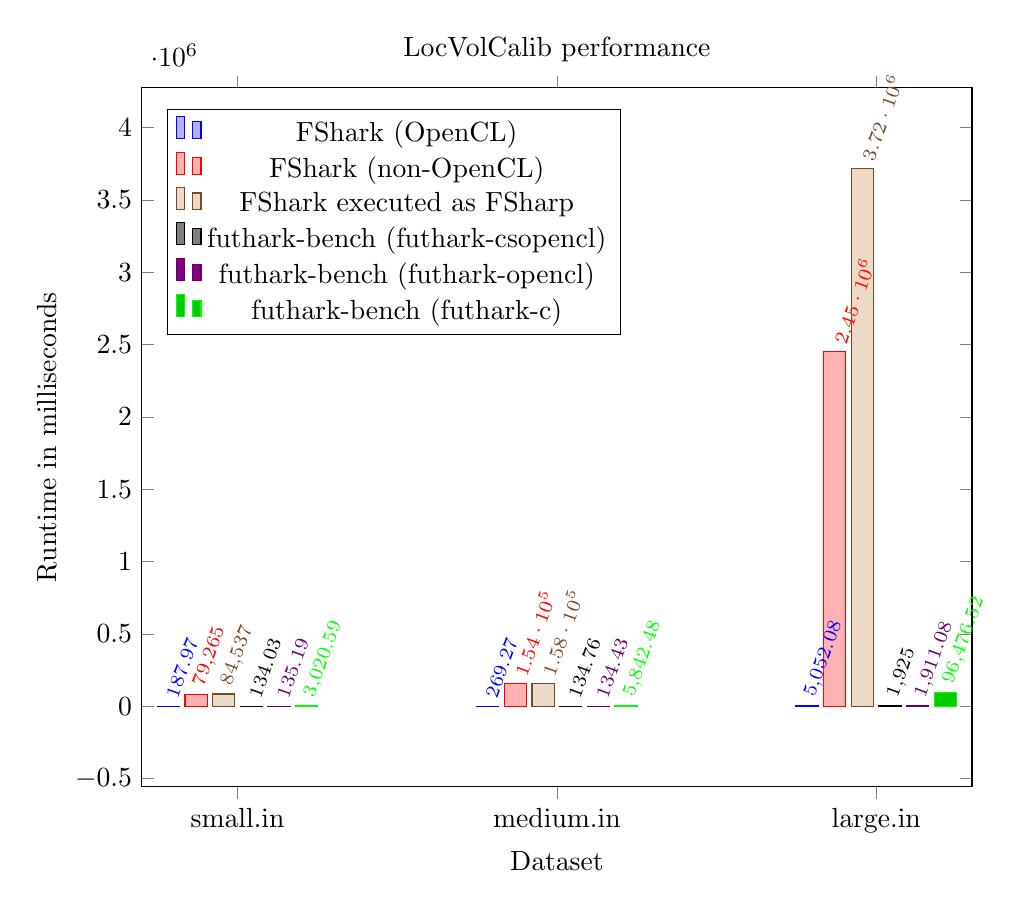
\begin{tikzpicture}
      \begin{axis}[
        title={LocVolCalib performance},
        xlabel={Dataset},
        ylabel={Runtime in milliseconds},
        width=1\textwidth,
        %height=0.5,
        symbolic x coords={small.in,medium.in,large.in},
        xtick=data,
        enlargelimits=0.15,
        ybar=2pt,% configures ‘bar shift’
        bar width=8pt,
        nodes near coords,
        every node near coord/.append style={rotate=70, anchor=west,font=\scriptsize},
        legend style={legend pos=north west}
      ]
      \addplot plot coordinates {(small.in, 187.972) (medium.in, 269.265 ) (large.in, 5052.080 )};
      \addplot plot coordinates {(small.in, 79265 ) (medium.in, 154488 ) (large.in, 2448660 )};

      \addplot plot coordinates {(small.in, 84537 ) (medium.in, 157735 ) (large.in, 3716097 )};

      \addplot plot coordinates {(small.in, 134.032 ) (medium.in, 134.761  ) (large.in,  1925.001 )};
      \addplot plot coordinates {(small.in, 135.192 ) (medium.in, 134.428 ) (large.in, 1911.079 )};
      \addplot plot coordinates {(small.in, 3020.588 ) (medium.in, 5842.482 ) (large.in, 96476.520 )};

      \legend{FShark (OpenCL), FShark (non-OpenCL), FShark executed as FSharp, futhark-bench (futhark-csopencl), futhark-bench (futhark-opencl), futhark-bench (futhark-c)}
      \end{axis}
    \end{tikzpicture}
    \caption{Comparison of LocVolCalib benchmark for multiple versions}
    \label{fig:line-graph}
\end{figure}

\section*{The \texttt{nbody} benchmark}

for all three datasets


\subsection*{Specifications for benchmark}
We have run the benchmarks on a system with these attributes:
\begin{itemize}
\item CPU: 4 cores of Intel Core i5-6500 at 3.20GHz
  \begin{itemize}
  \item L1 cache: 128 KiB 
  \item L2 cache: 1024 KiB 
  \item L3 cache: 6144 KiB 
  \end{itemize}
\item GPU: GeForce GTX 970
\end{itemize}


Introduction for the two benchmarks LocVolCalib and nbody



why are they faster in general




%%% Local Variables:
%%% mode: latex
%%% TeX-master: "../thesis"
%%% End: